\documentclass[border=10pt]{standalone}
\usepackage{tikz}\usepackage{amsmath}\usetikzlibrary{arrows.meta}
\begin{document}
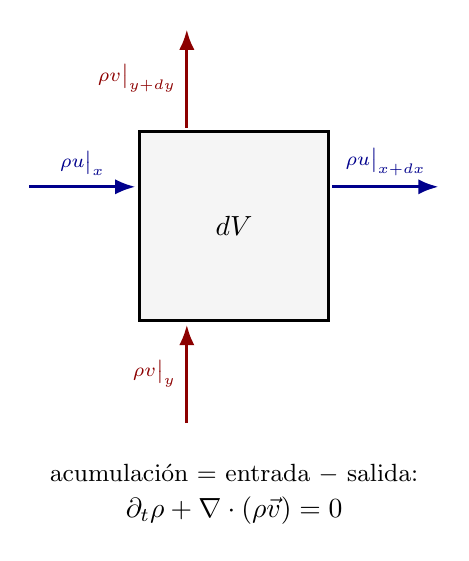
\begin{tikzpicture}[line width=0.9pt,>={Latex[length=2.6mm]}]
  \draw[fill=black!4] (0,0) rectangle (2.4,2.4);
  \node at (1.2,1.2){$dV$};
  % flujo entrante/saliente en x
  \draw[->,blue!55!black,line width=1.2pt] (-1.4,1.7)--(-0.05,1.7) node[midway,above]{\scriptsize$\rho u\big|_x$};
  \draw[->,blue!55!black,line width=1.2pt] (2.45,1.7)--(3.8,1.7) node[midway,above]{\scriptsize$\rho u\big|_{x+dx}$};
  % flujo en y
  \draw[->,red!55!black,line width=1.2pt] (0.6,-1.3)--(0.6,-0.05) node[midway,left]{\scriptsize$\rho v\big|_y$};
  \draw[->,red!55!black,line width=1.2pt] (0.6,2.45)--(0.6,3.7) node[midway,left]{\scriptsize$\rho v\big|_{y+dy}$};
  \node[align=center] at (1.2,-2.2){\small acumulación $=$ entrada $-$ salida:\\[1pt]$\partial_t\rho+\nabla\cdot(\rho\vec v)=0$};
\end{tikzpicture}
\end{document}
